\section{Macros}

\section{Notation}
\begin{itemize}
	\item By goal or problem or task we mean the overall task of the thesis, which is develop a machine learning model suitable for predicting prices on the financial market, based on a history of data.
\end{itemize}

\section{Datasets}
Here we describe the various datasets we used for the training and testing of our models. Each description includes the following:
\begin{itemize}
	\item \textbf{Source:} the name and source from where we took the dataset. Including a link or a way to access and download the dataset.
	\item \textbf{Collection method:} a description of how the data in the dataset was gathered and over what time span.
	\item \textbf{Motivation:} a description of what the data in the dataset represent, what their purpose is, how they were gathered and why it is valuable to our research.
	\item \textbf{Size:} a description of how many datapoints the dataset contains, how many features each datapoints has and the overall size of the file.
	\item \textbf{Features:} a description of the features each datapoint of the dataset has and what the features represent.
	\item \textbf{Quality:} a description of the features and drawbacks of the overall dataset e.g. how dependent are the features between themselves.
	\item \textbf{Plot:} a plot of the numeric features of the dataset, its visual representation.
\end{itemize}
\subsection{House sales}
\begin{itemize}
	\item \textbf{Source:} House Property Sales Time Series (raw\_sales.csv) :\\ https://www.kaggle.com/datasets/htagholdings/property-sales
	\item \textbf{Collection method:} Property sales data was gathered for the 2007-2019 period for one specific region.
	\item \textbf{Motivation:} A simple dataset for the easier models. A proper, manageable size, once filtered by property and number of bedrooms. Has very few features, making it easier to understand and process.
	\item \textbf{Size:} Consists of 29600 datapoints. Once filtered for property being house, number of bedrooms equal to 3, around 11300 datapoints remain.
	\item \textbf{Features:} The dataset has very few features. Every datapoint consists of:
	      \begin{itemize}
		      \item \textbf{datesold}: Date at which the sale was made.
		      \item \textbf{postcode}: 4 digit postcode of the suburb where the property was sold (given for reference only).
		      \item \textbf{price}: Price for which the property was sold.
		      \item \textbf{propertyType}: Property type i.e. house or unit.
		      \item \textbf{bedrooms}: Number of bedrooms: 1, 2, 3, 4 or 5.
	      \end{itemize}
	      The dataset was filtered by propertyType and bedrooms, and the postcode was discarded.
	\item \textbf{Quality:} The prices rise, while nonlinearly, with time.
	\item \textbf{Plot:}
	      \begin{figure}[h!]
		      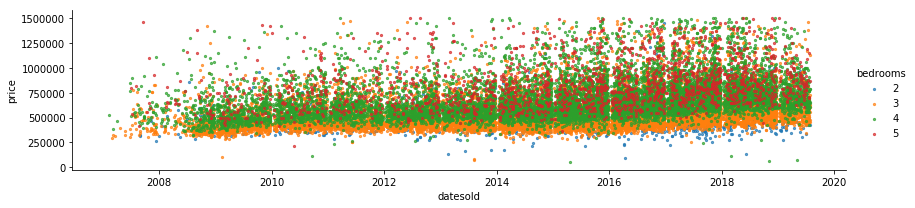
\includegraphics[width=\linewidth]{"pictures/house_sales_graph.png"}
		      \caption{A plot of the House Sales dataset.}
		      \label{fig:house_sales_graph}
	      \end{figure}
\end{itemize}
% \subsection{Gbpcad}
% \begin{itemize}
% 	\item \textbf{Source:}
% 	\item \textbf{Motivation:}
% 	\item \textbf{Size:}
% 	\item \textbf{Features:}
% 	\item \textbf{Collection method:}
% 	\item \textbf{Quality:}
% 	\item \textbf{Plot:}
% \end{itemize}
\subsection{Google Stock}
\begin{itemize}
	\item \textbf{Source:} Google Stock Dataset \\ https://www.kaggle.com/datasets/r1shabhgupta/google-stock-price-daily-weekly-and-monthly-2023/data
	\item \textbf{Collection method:} Collected from the stock market (probably). Has daily data and weekly and monthly summaries.
	\item \textbf{Motivation:} More complex dataset, multiple time series numeric features, but fewer datapoints.
	\item \textbf{Size:} Daily set has 2510 datapoints. Weekly set has 520 datapoints. Monthly set has 120 datapoints.
	\item \textbf{Features:} Every datapoint has the following features:
	      \begin{itemize}
		      \item \textbf{Date}: the date on which the stock price was recorded.
		      \item \textbf{Price}: the opening price of the stock on the given date.
		      \item \textbf{High}: the highest price at which the stock was traded during the day.
		      \item \textbf{Low}: the lowest price at which the stock was traded during the day.
		      \item \textbf{Close}: the closing price of the stock on the given date.
		      \item \textbf{Volume}: the total number of shares traded on the given date.
		      \item \textbf{Adj Close}: the adjusted closing price of the stock on the given date.
	      \end{itemize}
	\item \textbf{Quality:}
	\item \textbf{Plot:}
\end{itemize}
\subsection{Apple}
\begin{itemize}
	\item \textbf{Source:} Apple Stock Prices \\ https://www.kaggle.com/datasets/suyashlakhani/apple-stock-prices-20152020
	\item \textbf{Collection method:} Collected from the stock market (probably).
	\item \textbf{Motivation:} Even more features then the previous datasets, more interesting.
	\item \textbf{Size:} The dataset consists of 1258 datapoints.
	\item \textbf{Features:} Every datapoint has the following features
	      \begin{itemize}
		      \item \textbf{close} - Closing price
		      \item \textbf{high} - Highest price of the day
		      \item \textbf{low} - Lowest Price of the day
		      \item \textbf{open} - Opening price of the day
		      \item \textbf{volume} - Volume of stock traded
		      \item \textbf{adjClose} - Closing stock price in relation to other stock attributes/actions
		      \item \textbf{adjHigh} - Highest stock price in relation to other stock attributes/actions
		      \item \textbf{adjOpen} - Opening Stock price in relation to other stock attributes/actions
		      \item \textbf{adjVolume} - Trading volume in relation to other stock attributes/actions
		      \item \textbf{divCash} - Cash dividend
		      \item \textbf{splitFactor} - Stock split
	      \end{itemize}
	\item \textbf{Quality:}
	\item \textbf{Plot:}
\end{itemize}
\subsection{Gold}
\begin{itemize}
	\item \textbf{Source:} Gold rates \\ https://www.kaggle.com/datasets/hemil26/gold-rates-1985-jan-2022
	\item \textbf{Collection method:} This data was collected from https://www.gold.org/goldhub and then cleaned. Has daily data and annual summaries.
	\item \textbf{Motivation:} The dataset contains lots of datapoints and lots of features.
	\item \textbf{Size:} Annual dataset has 43 datapoints. Daily dataset has a bit over 10 thousand datapoints.
	\item \textbf{Features:} Each datapoint has the following features: date and rates in six curriencies: USD (American), INR (Indian), AED (Arabian), EUR (European), GBP (South Georgian) and CNY (Chinese).
	\item \textbf{Quality:}
	\item \textbf{Plot:}
\end{itemize}
\subsection{Electricity}
\begin{itemize}
	\item \textbf{Source:}
	\item \textbf{Motivation:}
	\item \textbf{Size:} The dataset has 26304 datapoints.
	\item \textbf{Features:} Each datapoint consists of a date and 320 numbered columns and an OT column.
	\item \textbf{Collection method:}
	\item \textbf{Quality:}
	\item \textbf{Plot:}
\end{itemize}
% \subsection{ETT-small}
% \begin{itemize}
% 	\item \textbf{Source:}
% 	\item \textbf{Motivation:}
% 	\item \textbf{Size:}
% 	\item \textbf{Features:}
% 	\item \textbf{Collection method:}
% 	\item \textbf{Quality:}
% 	\item \textbf{Plot:}
% \end{itemize}
% \subsection{Illness}
% \begin{itemize}
% 	\item \textbf{Source:}
% 	\item \textbf{Motivation:}
% 	\item \textbf{Size:}
% 	\item \textbf{Features:}
% 	\item \textbf{Collection method:}
% 	\item \textbf{Quality:}
% 	\item \textbf{Plot:}
% \end{itemize}
% \subsection{M4}
% \begin{itemize}
% 	\item \textbf{Source:}
% 	\item \textbf{Motivation:}
% 	\item \textbf{Size:}
% 	\item \textbf{Features:}
% 	\item \textbf{Collection method:}
% 	\item \textbf{Quality:}
% 	\item \textbf{Plot:}
% \end{itemize}
% \subsection{PEMS}
% \begin{itemize}
% 	\item \textbf{Source:}
% 	\item \textbf{Motivation:}
% 	\item \textbf{Size:}
% 	\item \textbf{Features:}
% 	\item \textbf{Collection method:}
% 	\item \textbf{Quality:}
% 	\item \textbf{Plot:}
% \end{itemize}
% \subsection{Prompt Bank}
% \begin{itemize}
% 	\item \textbf{Source:}
% 	\item \textbf{Motivation:}
% 	\item \textbf{Size:}
% 	\item \textbf{Features:}
% 	\item \textbf{Collection method:}
% 	\item \textbf{Quality:}
% 	\item \textbf{Plot:}
% \end{itemize}
% \subsection{Traffic}
% \begin{itemize}
% 	\item \textbf{Source:}
% 	\item \textbf{Motivation:}
% 	\item \textbf{Size:}
% 	\item \textbf{Features:}
% 	\item \textbf{Collection method:}
% 	\item \textbf{Quality:}
% 	\item \textbf{Plot:}
% \end{itemize}
% \subsection{Weather}
% \begin{itemize}
% 	\item \textbf{Source:}
% 	\item \textbf{Motivation:}
% 	\item \textbf{Size:}
% 	\item \textbf{Features:}
% 	\item \textbf{Collection method:}
% 	\item \textbf{Quality:}
% 	\item \textbf{Plot:}
% \end{itemize}
\subsection{Sine}
\begin{itemize}
	\item \textbf{Source:} sine.csv - we generated this dataset ourselves
	\item \textbf{Motivation:} This is a non-trivial, but predictable, dataset for testing whether LLM responds to the data.
	\item \textbf{Size:} Dataset consists of 1000 datapoints.
	\item \textbf{Features:} Each datapoint consists of date, x and target, where target = sin(x).
	\item \textbf{Collection method:} Dataset was generated by a script.
	\item \textbf{Quality:}
	\item \textbf{Plot:} A simple sine wave.
\end{itemize}

\section{What metrics we used}
Every metric should be described by
\begin{itemize}
	\item what it measures,
	\item how it is calculated,
	\item what its result represents,
	\item how valuable it is,
	\item when it can be applied.
\end{itemize}
\subsection{Mean Squared Error}

The Mean Squared Error (MSE) is a metric used for evaluating the accuracy of a machine learning model, especially in regression tasks. It quantifies how close a model's predictions are to the actual values.

\subsubsection{Definition}
MSE calculates the average of the squares of the errors. The error is the difference between the values (\(\hat{y}_i\)) predicted by the model and the values (\(y_i\)) it should have predicted.

\subsubsection{Calculation Steps}
The metric is computed as follows.
\begin{enumerate}
	\item For each prediction the error is computed by subtracting the predicted value from the actual value.
	\item Each error is then squared in order to ensure that positive and negative errors do not cancel each other out and in order to emphasize larger errors.
	\item The average of these squared errors is then computed to obtain the MSE.
\end{enumerate}

\subsubsection{Mathematical Formulation}
The mathematical formula for MSE is given by:
\begin{equation}
	MSE = \frac{1}{n} \sum_{i=1}^{n} (y_i - \hat{y}_i)^2
\end{equation}
where:
\begin{itemize}
	\item \(n\) is the number of data points,
	\item \(y_i\) is the actual value for the \(i\)th datapoint,
	\item \(\hat{y}_i\) is the predicted value for the \(i\)th datapoint,
\end{itemize}

\subsubsection{Interpretation}
\begin{itemize}
	\item MSE is a non-negative number where a value of 0 indicates perfect predictions.
	\item Larger MSE values indicate worse model performance.
	\item MSE emphasizes larger errors due to the squaring of each term, which can be both advantageous and disadvantageous depending on the application.
\end{itemize}

\subsection{R\(^2\) Score}

The \(R^2\) score, or the coefficient of determination, is a statistical measure used in regression analysis to assess how well fitted a model is. It indicates the proportion of the variance in the dependent variable that is predictable from the independent variable(s).

\subsubsection{Definition}
The \(R^2\) score is defined as the ratio of the variance explained by the model to the total variance. It is a measure of how well the observed outcomes are replicated by the model, based on the proportion of total variation of outcomes explained by the model.

\subsubsection{Calculation}
The \(R^2\) score is calculated using the following formula:
\begin{equation}
	R^2 = 1 - \frac{\sum_{i=1}^{n} (y_i - \hat{y}_i)^2}{\sum_{i=1}^{n} (y_i - \overline{y})^2}
\end{equation}
where:
\begin{itemize}
	\item \(y_i\) is the actual value for the \(i\)th data point,
	\item \(\hat{y}_i\) is the predicted value for the \(i\)th data point,
	\item \(\overline{y}\) is the mean of the actual values,
	\item \(n\) is the number of data points.
\end{itemize}

\subsubsection{Interpretation}
\begin{itemize}
	\item An \(R^2\) score of 1 indicates that the regression model perfectly fits the data.
	\item An \(R^2\) score of 0 means that the model does no better, than would a prediction using the mean.
	\item Negative \(R^2\) values can occur when the chosen model fits worse than a horizontal line representing the mean of the response.
\end{itemize}

\subsubsection{Limitations}
The \(R^2\) metric has some limitations. It does not necessarily imply causation, nor does a high \(R^2\) score mean that the model is the best choice for prediction. It's also important to note that adding more predictors to a model can artificially inflate the \(R^2\) value, even if those predictors are not statistically significant.


\section{How we describe models}
Below, in the chapter "Other models" we describe several models we tried to use for the task of predicting prices. The descriptions include the following:
\begin{itemize}
	% \item \textbf{Relevant literature:} 
	\item \textbf{Description:} a short description of how the model works and how it is trained.
	\item \textbf{Motivation:} what the model is usually used for and why we chose to try it out.
	\item \textbf{Features and limitations:} some advantages and benefits of the model, as well as its disadvantages and drawbacks.
	\item \textbf{Parameters:} the description of the parameters of the model and how they affect its training.
	\item \textbf{Metrics:} how we measured the results of the training and testing of the model.
	\item \textbf{Data used:} what combinations of parameters of the model we tested and on what datasets we trained and tested the model.
	\item \textbf{Preprocessing:} how the datasets used were preprocessed for training and testing of the model.
	\item \textbf{Analysis:} an analysis of our results of our training and testing of the model compared with the results obtained in literature.
	\item \textbf{Picture:} a picture or a plot demonstrating the results obtained from testing the model.
\end{itemize}

\section{Literature review}
Literature review contains:
\begin{itemize}
	\item A list of approaches to the problem.
	\item For each approach, its basic description and its significance to our goal.
	\item Its features and drawbacks compared to our goal.
	\item Its differences, when compared to our goal.
	\item Whether our own results validated the results of the article.
\end{itemize}

% notatki:
% opis modelu
% nasze wyniki vs. literatura
% dyskusja - krótka analiza, porównanie z literaturą

Dla LLM:
5 najciekawszych pomysłów, które zadziałały
5 najciekawszych pomysłów, które nie zadziałały

Kryteria oceniania:
czy nazwa odpowiada treści
czy ma wstęp, przegląd literatury, własną myśl itp.
czy jest jasno napisana
własne wnioski (dlaczego wydaje nam się, że to zadziałało, a to nie)

wyniki, które trochę przetrwają, coś ciekawego, coś, co ma uniwersalny charakter

co robić:
metryki, datasety
literature review - co tam ma być
